\begin{frame}
\begin{columns}[c]
\begin{column}{0.5\textwidth}
\begin{block}{\textbf{Observe gene expression}}
\begin{itemize}
\item examples of phenotypes: \begin{small}
1) transcript counts derived from RNA-seq data 2) qualitative organismal phenotypic characteristics such as coat color in mice or wing shape in flies
\end{small}
\item regardless of the level of observation the total number of \textbf{phenotype values} under consideration can be indexed as $P = \{ 1, \ldots, p \} $
\end{itemize}
\end{block}
\end{column}
\begin{column}{0.5\textwidth}
\begin{center}
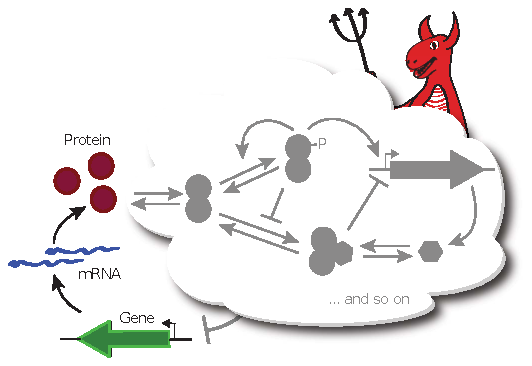
\includegraphics[width=1.0\textwidth]{fig/geneexpressiondemon.pdf}
\end{center}
\end{column}
\end{columns}
\end{frame}
